\end{multicols}
\begin{multicols}{2}[\section{The Application}]

%\emph{Description of our product. Features and the concept behind the UI. Possible improvements and add-ons.}

%\end{multicols}
%\begin{multicols}{2}[\subsection{Usability}]

%\emph{MyCourses} is able to create a semi-automatic scheduling for programs at universities or schools. It can also provide a scheduling that was run fully automatic but the recommended usage is to have \emph{MyCourses} create preliminary versions of a scheduling. These will then be improved by the users via the functionality for collaborative scheduling also provided by \emph{MyCourses}. This process is best used iteratively through several cycles of automatic assignment and manual improvement. To get better results from the automated scheduling users can define requirements and assign those to courses or resources. A requirement that is assigned to a course is regarded as a constraint that either must be met in case of a so called hard-constraint or simply improves the rating of a scheduling in case of a soft-constraint.

All in one the application provides the following functionality (illustration follows)

\begin{itemize}
\item login/logout and get detailed information about your personal profile

\item create, read, delete and modify data related to schedules

\item automatic validation of all forms

\item starting, resuming of schedulings with progress indicator

\item view timetables for a given room, a \emph{CourseInstance} and every user

\item import and export of course-related data

\item view courseinstance data and enroll in them

\item full accessibility on current browsers, even without JavaScript
\end{itemize}
\end{multicols}

\begin{figure}[t]
\setlength\fboxsep{0pt}
\setlength\fboxrule{0.5pt}
\fbox{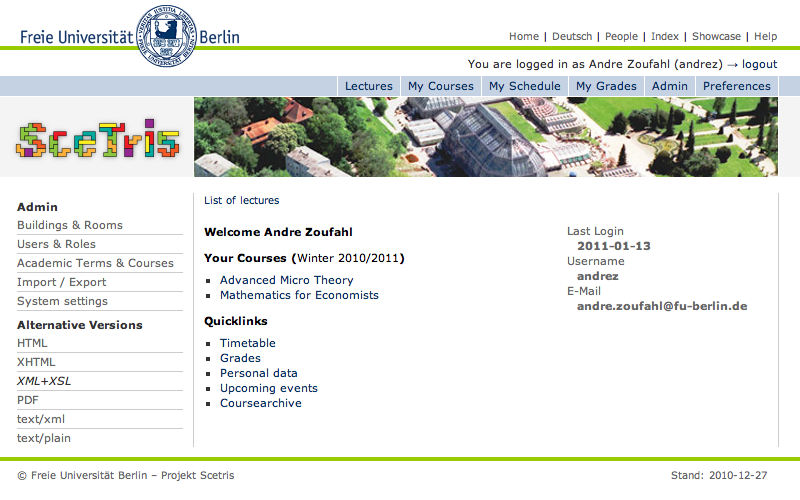
\includegraphics[width=\columnwidth]{images/app/start.png}} 
\caption{Basic layout of our application}%
\end{figure}

\begin{multicols}{2}

\begin{figure}[H]
\fbox{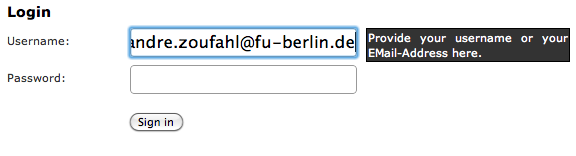
\includegraphics[width=\columnwidth]{images/app/login.png}}%
\caption{Login: input fields provide user with information on what to fill in}%
\end{figure}

\begin{figure}[H]
\fbox{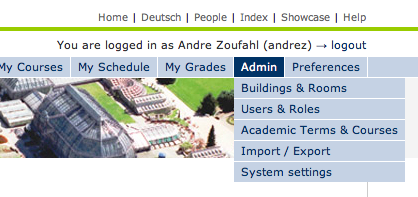
\includegraphics[width=\columnwidth]{images/app/login_after.png}}%
\caption{Login status is tracked on every page. Navigation provides submenus when hovering over items.}%
\end{figure}

\end{multicols}
\begin{multicols}{2}

\begin{figure}[H]
\fbox{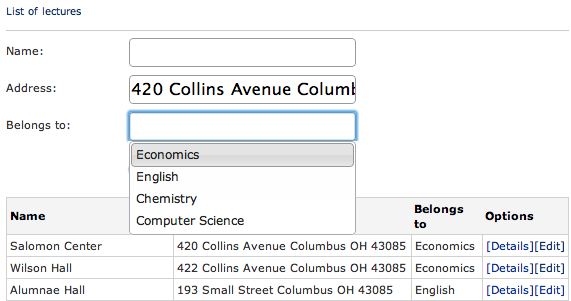
\includegraphics[width=\columnwidth]{images/app/building_list.png}}%
\caption{With JavaScript activated selections morph into textfields with automatic proposals.}%
\end{figure}

\begin{figure}[H]
\fbox{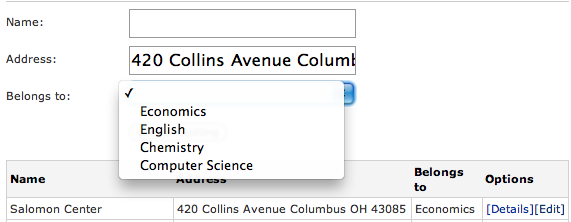
\includegraphics[width=\columnwidth]{images/app/building_list_nojs.png}}%
\caption{Without JavaScript the standard selection is used.}%
\end{figure}

\end{multicols}
\begin{multicols}{2}

\begin{figure}[H]
\fbox{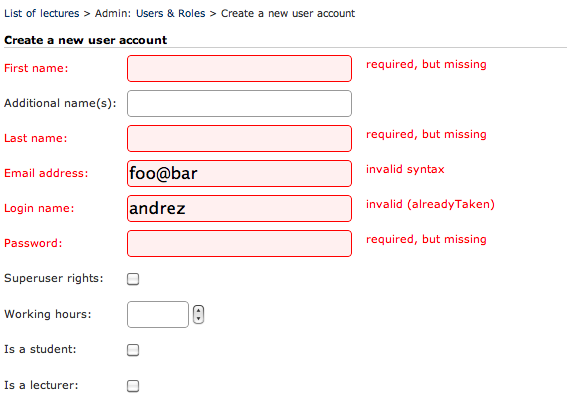
\includegraphics[width=\columnwidth]{images/app/forms_invalid.png}}%
\caption{Form validation: no data can be send until all problems were solved.}%
\end{figure}

\begin{figure}[H]
\fbox{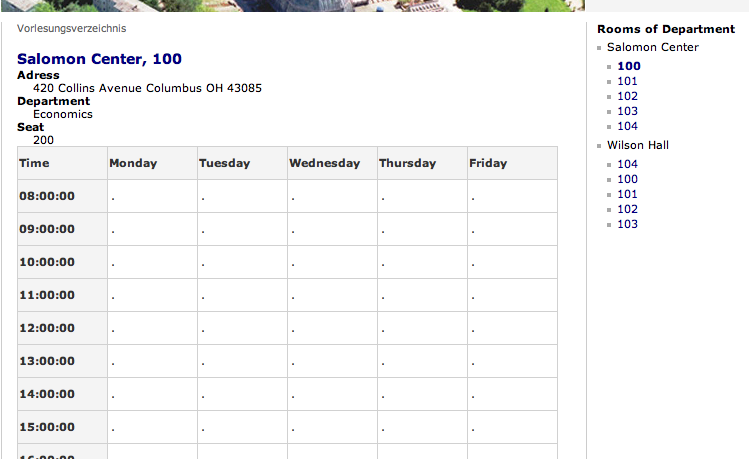
\includegraphics[width=\columnwidth]{images/app/timetable_empty.png}}%
\caption{Before scheduling: CourseElementInstances have no time or room assigned, all rooms are free.}%
\end{figure}

\end{multicols}
\begin{multicols}{2}

\begin{figure}[H]
\fbox{
\includegraphics[width=\columnwidth]{images/app/scheduler_start.png}}%
\caption{If the scheduler is not running, it's possible to schedule the academic term for a given department.}%
\end{figure}

\begin{figure}[H]
\fbox{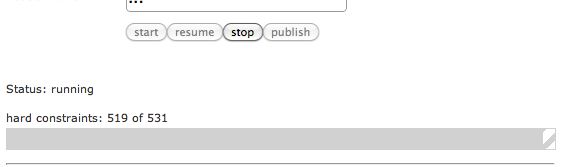
\includegraphics[width=\columnwidth]{images/app/scheduler_running.png}}%
\caption{A progress bar indicates how many constraints are already solved.}%
\end{figure}

\end{multicols}
\begin{multicols}{2}

\begin{figure}[H]
\fbox{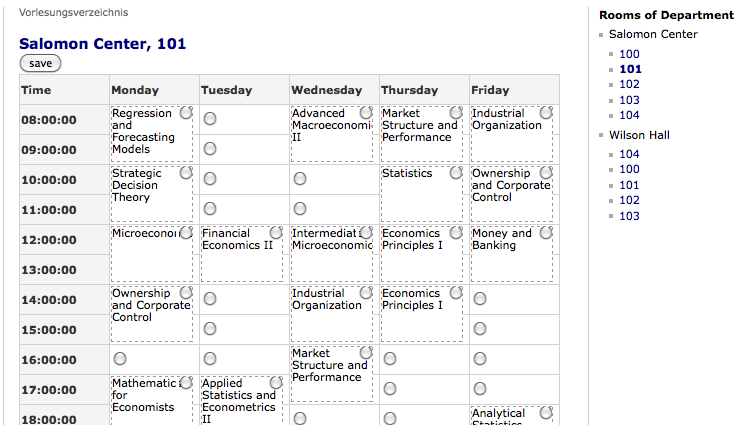
\includegraphics[width=\columnwidth]{images/app/timetable_edit.png}}%
\caption{Manual changes: after scheduling the program manager can also swap positions of courses.}%
\end{figure}

\begin{figure}[H]
\fbox{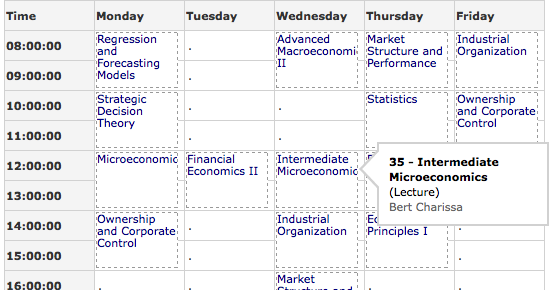
\includegraphics[width=\columnwidth]{images/app/timetable_final.png}}%
\caption{After scheduling: every room contains several CourseElementInstances. Hovering over an event provides the user with data about the event as well as a direct link to the related CourseInstance.}%
\end{figure}

\end{multicols}
\pagebreak
\begin{multicols}{2}

\begin{figure}[H]
\fbox{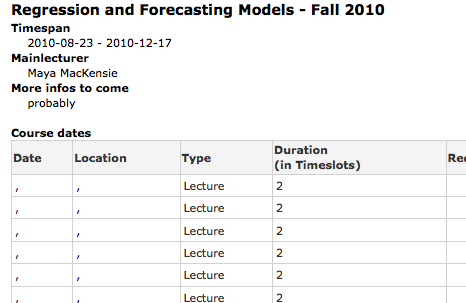
\includegraphics[width=\columnwidth]{images/app/coursedetail_empty.png}}%
\caption{Before publishing of the scheduling every CourseInstance may be inspected but has no dates for their CourseElementInstances.}%
\end{figure}

\begin{figure}[H]
\fbox{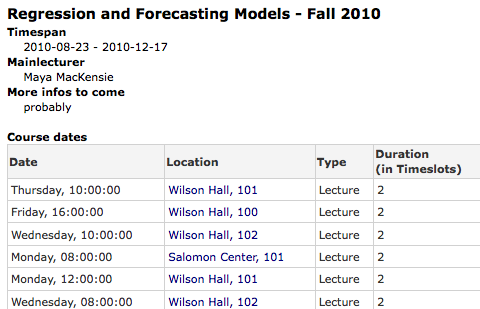
\includegraphics[width=\columnwidth]{images/app/coursedetail_published.png}}%
\caption{After the program manager published and freezed the scheduling it is possible to enroll on any given CourseInstance.}%
\end{figure}

\end{multicols}
\begin{multicols}{2}

\begin{figure}[H]
\fbox{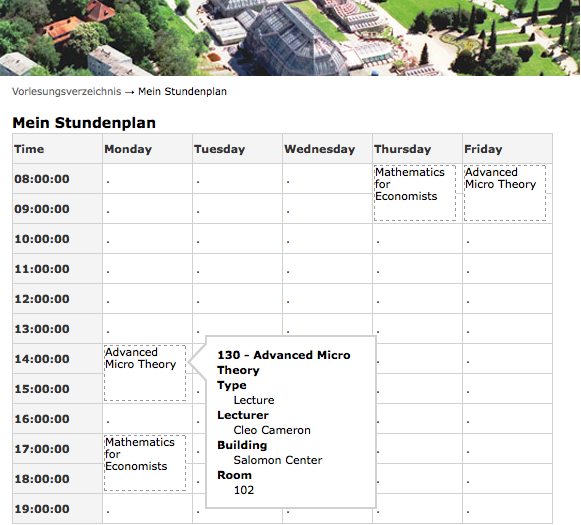
\includegraphics[width=\columnwidth]{images/app/mytimetable.png}}%
\caption{Once the user enrolls in some CourseInstances the user can view its personal timetable for the week.}%
\end{figure}
